\chapter{Tools}
\label{tools}

\index{IDE}

The steps for compiling, running, and debugging Java code depend on your development environment and operating system.
We avoided putting these details in the main text, because they can be distracting.
Instead, we provide this appendix with a brief introduction to DrJava---an {\bf integrated development environment} (IDE) that is helpful for beginners---and other development tools, including Checkstyle for code quality and JUnit for testing.


\section{Installing DrJava}
\label{drjava}

The easiest way to start programming in Java is to use a website that compiles and runs Java code in the browser.
Examples include \url{https://repl.it/}, \url{https://trinket.io/}, \url{https://jdoodle.com/}, and others.

If you are unable to install software on your computer (which is often the case in public schools and Internet caf\'{e}s), you can use these online development environments for almost everything in this book.

But if you want to compile and run Java programs on your own computer, you will need:

\begin{itemize}

\item The {\bf Java Development Kit} (JDK), which includes the compiler, the {\bf Java Virtual Machine} (JVM) that interprets the compiled byte code, and other tools such as Javadoc.

\index{JDK}
\index{JVM}
\index{virtual machine}
\index{Javadoc}

\index{text editor}
\index{DrJava}

\item A {\bf text editor} such as Atom, Notepad++, or Sublime Text, and/or an IDE such as DrJava, Eclipse, jGrasp, or NetBeans.

\end{itemize}

The JDK we recommend is OpenJDK, an open-source implementation of Java~SE (Standard Edition).
The IDE we recommend is DrJava, which is an open-source development environment written in Java (see Figure~\ref{fig.drjava1}).

To install OpenJDK, visit \url{https://adoptopenjdk.net}.
Download and run the installer for your operating system.

%To install the JDK, search the web for ``download JDK'' which should take you to Oracle's website.
%Scroll down to ``Java Platform, Standard Edition'' and click the download button under JDK.
%Then accept the license agreement and select the installer for your operating system.
%Don't forget to run the installer after you download it!

\index{JAR}

% TODO: ML suggest pointing to an installation video (or making one)

To install DrJava, visit \url{http://drjava.org/} and download the {\bf JAR} file.
We recommend that you save it to your Desktop or another convenient location.
Simply double-click the JAR file to run DrJava.
Refer to the DrJava documentation (\url{http://drjava.org/docs/quickstart/}) for more details.

\begin{figure}[!ht]
\begin{center}
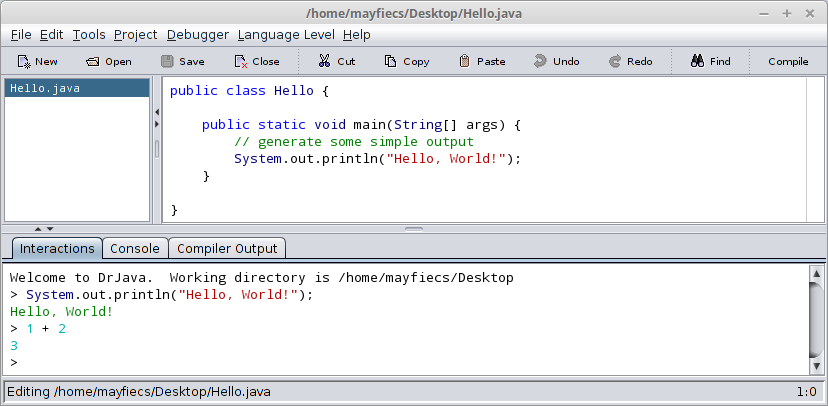
\includegraphics[width=0.95\textwidth]{figs/drjava-hello.png}
\caption{Screenshot of DrJava editing the hello world program.}
\label{fig.drjava1}
\end{center}
\end{figure}

When running DrJava for the first time, we recommend you change three settings from the {\sf Edit $>$ Preferences} menu under {\sf Miscellaneous}: set the {\sf Indent Level} to 4, check the {\sf Automatically Close Block Comments} box, and uncheck the {\sf Keep Emacs-style Backup Files} box.

%We will use DrJava as the primary development environment throughout this book.

%Step-by-step instructions for installing the JDK and configuring DrJava are available on this book's website: \url{https://thinkjava.org/}.


\section{DrJava Interactions}
\label{interactions}

One of the most useful features of DrJava is the ``Interactions Pane'' at the bottom of the window.
It provides the ability to try out code quickly, without having to write a class definition and save/compile/run the program.
Figure~\ref{fig.drjava2} shows an example.

\index{interactions}

\begin{figure}[!ht]
\begin{center}
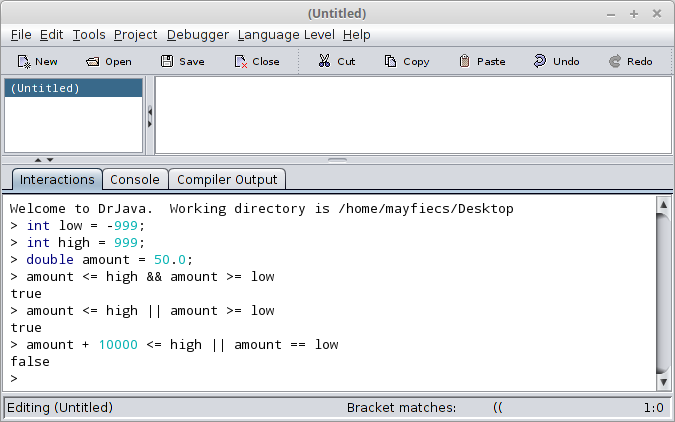
\includegraphics[width=0.95\textwidth]{figs/drjava-logic.png}
\caption{Screenshot of the Interactions Pane in DrJava.}
\label{fig.drjava2}
\end{center}
\end{figure}

There is one subtle detail to note when using the Interactions feature.
If you don't end an expression (or statement) with a semicolon, DrJava automatically displays its value.
Notice in Figure~\ref{fig.drjava2} how the variable declarations end with semicolons, but the logic expressions in the following lines do not.
This feature saves you from having to type \java{System.out.println} every time.

What's nice about this feature is that you don't have to create a new class, declare a \java{main} method, write arbitrary expressions inside \java{System.out.println} statements, save the source file, and get all of your code to compile in advance.
Also, you can press the up/down arrows on the keyboard to repeat previous commands and experiment with incremental differences.


\section{Command-Line Interface}
\label{commandline}

\index{command-line interface}
\index{terminal}

One of the most powerful and useful skills you can learn is how to use the {\bf command-line interface}, also called the ``terminal''.
The command line is a direct interface to the operating system.
It allows you to run programs, manage files and directories, and monitor system resources.
Many advanced tools, both for software development and general-purpose computing, are available only at the command line.

There are many good tutorials online for learning the command line for your operating system; just search the web for ``command line tutorial''.
On Unix systems like Linux and OS X, you can get started with just four commands: change the working directory ({\tt cd}), list directory contents ({\tt ls}), compile Java programs ({\tt javac}), and run Java programs ({\tt java}).

Figure~\ref{fig.terminal} shows an example where the {\tt Hello.java} source file is stored in the {\tt Desktop} directory.
After changing to that location and listing the files, we use the {\tt javac} command to compile {\tt Hello.java}.
Running {\tt ls} again, we see that the compiler generated a new file, {\tt Hello.class}, which contains the byte code.
We run the program using the {\tt java} command, which displays the output on the following line.

\begin{figure}[!ht]
\begin{center}
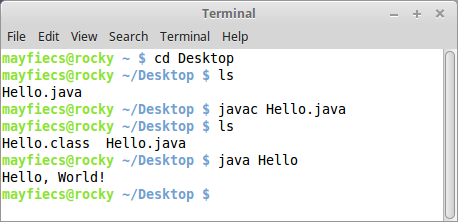
\includegraphics[width=4.5in]{figs/terminal.png}
\caption{Compiling and running {\tt Hello.java} from the command line.}
\label{fig.terminal}
\end{center}
\end{figure}

Note that the {\tt javac} command requires a {\em filename} (or multiple source files separated by spaces), whereas the {\tt java} command requires a single {\em class name}.
If you use DrJava, it runs these commands for you behind the scenes and displays the output in the Interactions Pane.

Taking time to learn this efficient and elegant way of interacting with the operating system will make you more productive.
People who don't use the command line don't know what they're missing.


\section{Command-Line Testing}
\label{cltesting}

\index{testing}

As described in Section~\ref{sec:examples}, it's more effective to program and debug your code little by little than to attempt writing everything all at once.
And after you've completed programming an algorithm, it's important to test that it works correctly on a variety of inputs.

Throughout the book, we illustrate techniques for testing your programs.
Most, if not all, testing is based on a simple idea: does the program do what we expect it to do?
For simple programs, it's not difficult to run them several times and see what happens.
But at some point, you will get tired of typing the same test cases over and over.

We can automate the process of entering input and comparing ``expected output'' with ``actual output'' using the command line.
The basic idea is to store the test cases in plain text files and trick Java into thinking they are coming from the keyboard.
Here are step-by-step instructions:

\begin{enumerate}

\item Make sure you can compile and run the {\tt Convert.java} example in the {\tt ch03} directory of {\tt ThinkJavaCode2}.
(See page~\pageref{code} for instructions on how to download the repository.)

\item In the same directory as {\tt Convert.java}, create a plain text file named {\tt test.in} (``in'' is for input).
Enter the following line and save the file:

\begin{stdout}
193.04
\end{stdout}

\item Create a second plain text file named {\tt test.exp} (``exp'' is for expected).
Enter the following line and save the file:

\begin{stdout}
193.04 cm = 6 ft, 4 in
\end{stdout}

\item Open a terminal, and change to the directory with these files.
Run the following command to test the program:

\begin{stdout}
java Convert < test.in > test.out
\end{stdout}

\end{enumerate}

\index{redirection operator}
\index{operator!redirection}
\index{System.in}
\index{System.out}

On the command line, {\tt <} and {\tt >} are {\bf redirection operators}.
The first one redirects the contents of {\tt test.in} to \java{System.in}, as if it were entered from the keyboard.
The second one redirects the contents of \java{System.out} to a new file {\tt test.out}, much like a screen capture.
In other words, the {\tt test.out} file contains the output of your program.

By the way, it's perfectly okay to compile your programs in DrJava (or some other environment) and run them from the command line.
Knowing both techniques allows you to use the right tool for the job.

% CSM: moving fig.meld here so it's not in the middle of Checkstyle

\begin{figure}[!ht]
\begin{center}
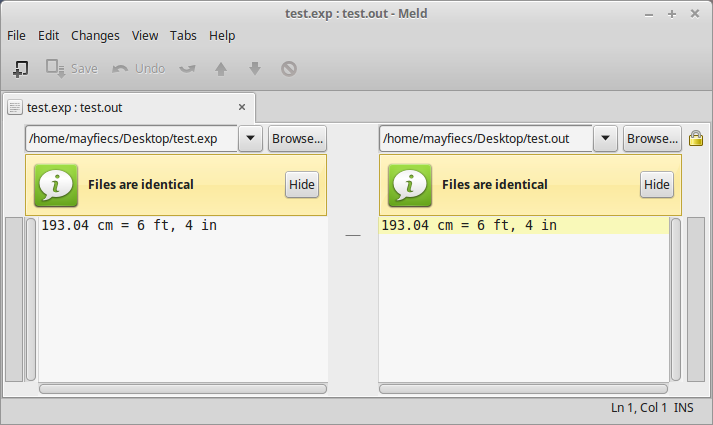
\includegraphics[width=0.95\textwidth]{figs/meld.png}
\caption{Using {\tt meld} to compare expected output with the actual output.}
\label{fig.meld}
\end{center}
\end{figure}

At this point, we just need to compare the contents {\tt test.out} with {\tt test.exp}.
If the files are the same, then the program outputted what we expected it to output.
If not, then we found a bug, and we can use the output to begin debugging our program.
Fortunately, there's a simple way to compare files on the command line:

\begin{stdout}
diff test.exp test.out
\end{stdout}

The {\tt diff} utility summarizes the differences between two files.
If there are no differences, then it displays nothing, which in our case is what we want.
If the expected output differs from the actual output, then we need to continue debugging.
Usually the program is at fault, and {\tt diff} provides some insight about what is broken.
But there's also a chance that we have a correct program and the expected output is wrong.

Interpreting the results from {\tt diff} can be confusing, but fortunately there are many graphical tools that show the differences between two files.
For example, on Windows you can install {\tt WinMerge}, on Mac you can use {\tt opendiff} (which comes with Xcode), and on Linux there's {\tt meld}, shown in Figure~\ref{fig.meld}.

Regardless of what tool you use, the goal is the same.
Debug your program until the actual output is {\em identical} to the expected output.


\section{Running Checkstyle}
\label{checkstyle}

\index{Checkstyle}

Checkstyle is a command-line tool that can be used to determine if your source code follows a set of style rules.
It also checks for common programming mistakes, such as class and method design problems.

You can download the latest version as a JAR file from \url{https://checkstyle.sourceforge.io/}.
To run Checkstyle, move (or copy) the JAR file to the same directory as your program.
Open a terminal in that location, and run the following command:

\begin{stdout}
java -jar checkstyle-*-all.jar -c /google_checks.xml *.java
\end{stdout}

\index{wildcard}

The {\tt *} characters are {\bf wildcards} that match whatever version of Checkstyle you have and whatever Java source files are present.
The output indicates the file and line number of each problem.
This example refers to a method beginning on line 93, column 5 of {\tt Hello.java}:

\begin{stdout}
Hello.java:93:5: Missing a Javadoc comment
\end{stdout}

The file \java{/google_checks.xml} is inside the JAR file and represents most of Google's style rules.
You can alternatively use \java{/sun_checks.xml} or provide your own configuration file.
See Checkstyle's website for more information.

If you apply Checkstyle to your source code often, you will likely internalize good style habits over time.
But there are limits to what automatic style checkers can do.
In particular, they can't evaluate the {\em quality} of your comments, the {\em meaning} of your variable names, or the {\em structure} of your algorithms.

Good comments make it easier for experienced developers to identify errors in your code.
Good variable names communicate the intent of your program and how the data is organized.
And good programs are designed to be efficient and demonstrably correct.


\section{Tracing with a Debugger}
\label{debugger}

\index{debugger}

A great way to visualize the flow of execution, including how parameters and arguments work, is to use a {\bf debugger}.
Most debuggers make it possible to:

\index{breakpoint}

\begin{enumerate}
\item Set a {\bf breakpoint}, a line where you want the program to pause.
\item Step through the code one line at a time and watch what it does.
\item Check the values of variables and see when and how they change.
\end{enumerate}

For example, open any program in DrJava and move the cursor to the first line of \java{main}.
Press {\sf Ctrl+B} to toggle a breakpoint on the current line; it should now be highlighted in red.
Press {\sf Ctrl+Shift+D} to turn on Debug Mode; a new pane should appear at the bottom of the window.
These commands are also available from the {\sf Debugger} menu, in case you forget the shortcut keys.

\index{call stack}

When you run the program, execution pauses at the first breakpoint.
The debug pane displays the {\bf call stack}, with the current method on top of the stack, as shown in Figure~\ref{fig.debugger}.
You might be surprised to see how many methods were called before the \java{main} method!

\begin{figure}[!ht]
\begin{center}
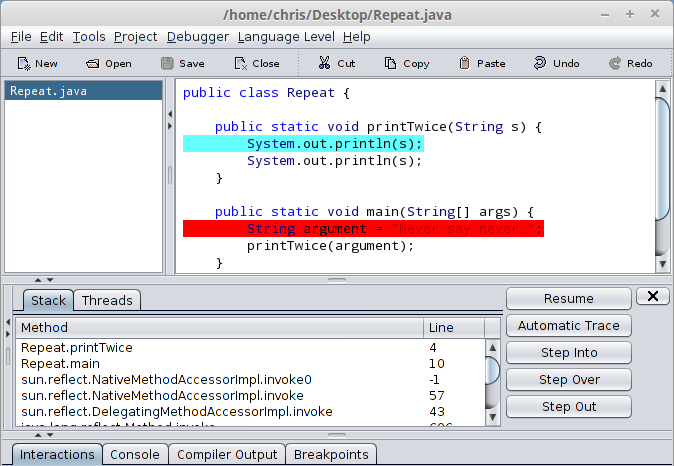
\includegraphics[width=0.95\textwidth]{figs/debugger.png}
\caption{Screenshot of the DrJava debugger.
Execution is currently paused on the first line of \java{printTwice}.
There is a breakpoint on the first line of \java{main}.}
\label{fig.debugger}
\end{center}
\end{figure}

%TODO: Production issue: the \java inside a caption is a problem for DocBook.

\index{tracing}

To the right are several buttons that allow you to step through the code at your own pace.
You can also press {\sf Automatic Trace} to watch DrJava run your code one line at a time.

Using a debugger is like having the computer proofread your code out loud.
When the program is paused, you can examine (or even change) the value of any variable using the Interactions Pane.

Tracing allows you to follow the flow of execution and see how data pass from one method to another.
You might expect the code do one thing, but then the debugger shows it doing something else.
At that moment, you gain insight about what may be wrong with the code.

You can edit your code while debugging it, but we don't recommend it.
If you add or delete multiple lines of code while the program is paused, the results can be confusing.

See \url{http://drjava.org/docs/user/ch09.html} for more information about using the debugger feature of DrJava.


\section{Testing with JUnit}
\label{JUnit}

\index{unit test}

When beginners start writing methods, they usually test them by invoking them from \java{main} and checking the results by hand.
%Writing code like this can get repetitive, but there are tools to make it easier.
For example, to test \java{fibonacci} from Section~\ref{fibonacci}, we could write:

\begin{code}
public static void main(String[] args) {
    if (fibonacci(1) != 1) {
        System.err.println("fibonacci(1) is incorrect");
    }
    if (fibonacci(2) != 1) {
        System.err.println("fibonacci(2) is incorrect");
    }
    if (fibonacci(3) != 2) {
        System.err.println("fibonacci(3) is incorrect");
    }
}
\end{code}

This test code is self-explanatory, but it's longer than it needs to be, and it doesn't scale very well.
In addition, the error messages provide limited information.
%Using a unit test framework addresses these and other issues.
For cases where we know the right answer, we can do better by writing {\bf unit tests}.


JUnit is a common testing tool for Java programs (see \url{https://junit.org/}).
To use it, you have to create a test class that contains test methods.

For example, suppose that the \java{fibonacci} method belongs to a class named \java{Series}.
Here is the corresponding JUnit test class and test method:

\begin{code}
import junit.framework.TestCase;

public class SeriesTest extends TestCase {

    public void testFibonacci() {
        assertEquals(1, Series.fibonacci(1));
        assertEquals(1, Series.fibonacci(2));
        assertEquals(2, Series.fibonacci(3));
    }
}
\end{code}

This example uses the keyword \java{extends}, which indicates that the new class, \java{SeriesTest} is based on an existing class, \java{TestCase}.
The \java{TestCase} class is imported from the package \java{junit.framework}.

The names in this example follow convention: if the name of your class is \java{Something}, the name of the test class should be \java{SomethingTest}.
And if there is a method in \java{Something} named \java{someMethod}, there should be a method in \java{SomethingTest} named \java{testSomeMethod}.

Many development environments can generate test classes and test methods automatically.
In DrJava, you can select {\sf New JUnit Test Case} from the {\sf File} menu to generate an empty test class.

\java{assertEquals} is provided by the \java{TestCase} class.
It takes two arguments and checks whether they are equal.
If so, it does nothing; otherwise it displays a detailed error message.
The first argument is the ``expected value'', which we consider correct, and the second argument is the ``actual value'' we want to check.
If they are not equal, the test fails.

\index{System.err}

Using \java{assertEquals} is more concise than writing your own \java{if} statements and \java{System.err} messages.
JUnit provides additional assert methods, such as \java{assertNull}, \java{assertSame}, and \java{assertTrue}, that can be used to design a variety of tests.

To run JUnit directly from DrJava, click the {\sf Test} button on the toolbar.
If all your test methods pass, you will see a green bar in the lower-right corner.
Otherwise, DrJava will take you directly to the first assertion that failed.


\section{Vocabulary}

\begin{description}

\term{IDE}
An ``integrated development environment'' that includes tools for editing, compiling, and debugging programs.

\term{JDK}
The ``Java Development Kit'' that contains the compiler, Javadoc, and other tools.

\term{JVM}
The ``Java Virtual Machine'' that interprets the compiled byte code.

\term{text editor}
A program that edits plain text files, the format used by most programming languages.

\term{JAR}
A ``Java Archive'', which is essentially a ZIP file containing classes and other resources.

\term{command-line interface}
A means of interacting with the computer by issuing commands in the form of successive lines of text.

\term{redirection operator}
A command-line feature that substitutes \java{System.in} and/or \java{System.out} with a plain text file.

\term{wildcard}
A command-line feature that allows you to specify a pattern of filenames using the {\tt *} character.

\term{debugger}
A tool that allows you to run one statement at a time and see the contents of variables.

\term{breakpoint}
A line of code where the debugger will pause a running program.

\term{call stack}
The history of method calls and where to resume execution after each method returns.

\term{unit test}
Code that exercises a single method of a program, testing for correctness and/or efficiency.

\end{description}
